\section{Adafruit Bonnet}

All inputs and outputs are managed through the Adafruit 1.3" Color TFT Bonnet for Raspberry Pi \cite{adafruitwebsite}. This bonnet includes a 240x240 pixel TFT display, a joystick, and two buttons. The button inputs are read through a standard GPIO interface, while the display is driven by the ST7789V chip connected via SPI.

To integrate the Adafruit Bonnet, example files were created to test its functionality and ensure compatibility with the board.

\subsection{Buttons}

\paragraph{Implementation:}
Making the buttons functional was straightforward thanks to the \texttt{example\_gpio\_intr} application from the x-heep repository \cite{xHeepRepo}, which served as a template.

There are six buttons in total: a joystick on the left side of the display (UP, DOWN, LEFT, and RIGHT), and two buttons (A and B) on the right side of the display. These buttons are read by polling the GPIO pins, which aligns with DOOM's input handling via polling.

\subsection{Display Driver Development}

As DOOM works by filling a screenbuffer, that is then sent to the display, the functionnality we need from the display are rudimentary. It needs to be able to fill entirely or in a fixed rectangle with pixels provided from the microcontroller.

Making the display work, however, was more complex than expected. The Adafruit Bonnet is designed as a Raspberry Pi HAT, with its original driver written in Python. The ST7789 chip, common in TFT displays, has several existing driver implementations. For this project, the Arduino ST7789 Fast library on GitHub \cite{arduinoST7789} was used as a reference.

\subsubsection*{Communication with the Display}


The ST7789 communicates with the board via an SPI interface, typically involving the following pins:
\begin{itemize}
\item \textbf{MOSI (Master Out Slave In):} Data lane from master to slave.
\item \textbf{MISO (Master In Slave Out):} Data lane from slave to master (not used by ST7789).
\item \textbf{SCK (Serial Clock):} Synchronizes data transfer, active only during transfer.
\item \textbf{CS (Chip Select):} Selects the slave device, active low.
\end{itemize}
Additionally, the ST7789 uses a \textbf{DC (Data/Command)} line, where high indicates data and low indicates commands.

In the x-Heep implementation on the PYNQ-Z2 FPGA, the SPI interface is pre-implemented. However, the SPI interface cannot send the DC signal, which must be sent separately using a GPIO pin. Initially, displaying information required sending the initialization sequence from an Arduino, then switching the cables to the board. Debugging with a logic analyzer revealed timing issues due to asynchronous SPI and synchronous DC pin operations. Adding a delay each time the DC pin changes state resolved this, ensuring proper signal synchronization.

This issue significantly delayed the project, compounded by a faulty initial display unit.

\begin{figure}[ht]
    \centering
    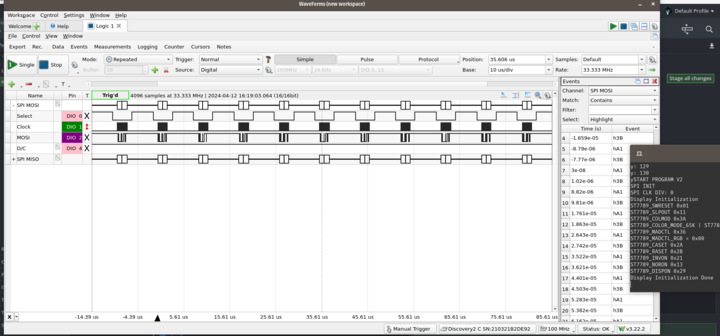
\includegraphics[width=0.6\textwidth]{images/Logic_analyzer_zoom_out.png}
    \caption{Overview of the display initialization sequence.}
    \label{fig:Logic_analyzer_zoom_out}
    \vspace{0.5cm}
    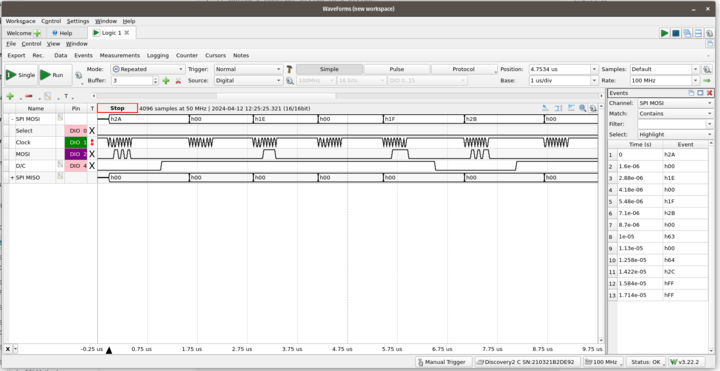
\includegraphics[width=0.6\textwidth]{images/Logic_analyzer_zoom_in.png}
    \caption{Detailed view of the display initialization sequence.} 
    \label{fig:Logic_analyzer_zoom_in}
\end{figure}

\subsection{Pinout Configuration}

On the PYNQ-Z2 FPGA, the buttons are connected to the following pins:

\begin{table}[ht]
    \centering
    \begin{tabular}{|c|c|c|c|}
        \hline
        \textbf{Description} & \textbf{PYNQ-Z2 PIN} & \textbf{Physical Location} & \textbf{Software PIN} \\
        \hline
        \hline
        Joystick UP & U8 & Raspberry Pi 15 & GPIO 9 \\
        \hline
        Joystick DOWN & V7 & Raspberry Pi 13 & GPIO 10 \\
        \hline
        Joystick LEFT & U7 & Raspberry Pi 11 & GPIO 11 \\
        \hline
        Joystick RIGHT & V6 & Raspberry Pi 8 & GPIO 12 \\
        \hline
        Button A & U13 & Arduino AR2 & GPIO 13 \\
        \hline
        Button B & V13 & Arduino AR3 & GPIO 14 \\
        \hline
        \hline
        Display CLK & H15 & Arduino SPI 3 & spi\_sck\_o \\
        \hline
        Display MOSI & T12 & Arduino SPI 4 & spi\_sd\_io[0] \\
        \hline
        Display CS & F16 & Arduino SPI 5 & spi\_csb\_o \\
        \hline
        Display DC & V8 & Raspberry Pi 19 & GPIO 8 \\
        \hline
    \end{tabular}
    \caption{Overview of the connections between the PYNQ-Z2 FPGA and the Adafruit Bonnet}
    \label{table:pinout_Adafruit}
\end{table}